% A faire, fin de chapitre 4


\documentclass{report}
\usepackage{filecontents}

\usepackage[utf8]{inputenc}
\usepackage[T1]{fontenc}
\usepackage[francais]{babel}
\usepackage{listings}
\usepackage[a4paper]{geometry}
\usepackage{graphicx}
\usepackage[export]{adjustbox}
\usepackage{titlesec}
\usepackage{color}
\usepackage[toc, page]{appendix}
\usepackage{url}

\definecolor{xcodekw}{rgb}{0.75, 0.22, 0.60}
\definecolor{xcodestr}{rgb}{0.89, 0.27, 0.30}
\definecolor{xcodecmt}{rgb}{0.31, 0.73, 0.35}

\titleformat{\chapter}[display]
  {\centering\normalfont\huge\bfseries}
  {\chaptertitlename\ \thechapter}
  {20pt}
  {\Huge}

\geometry{hscale=0.75,vscale=0.85,centering}

\renewcommand{\thesection}{\arabic{section}}
\renewcommand\appendixtocname{Annexes}
\renewcommand\appendixname{Annexes}
\renewcommand\appendixpagename{Annexes}

\title{Administration\\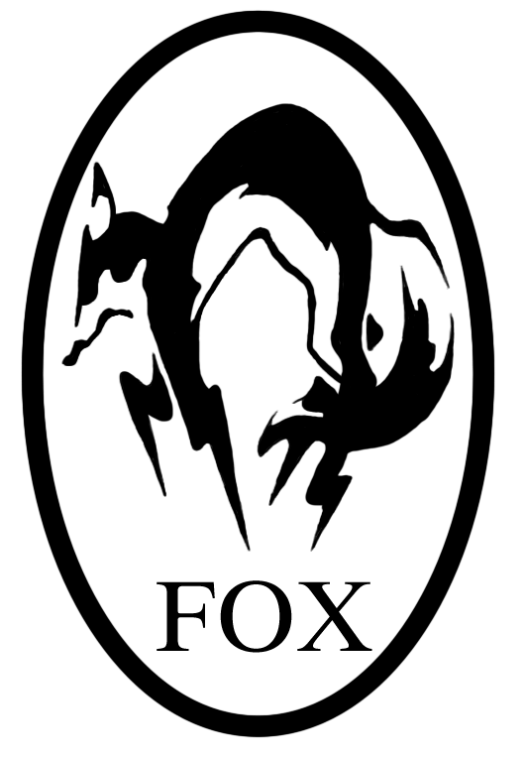
\includegraphics[scale=0.3]{foxhound.png}}
\author{Samuel "Big Boss" \bsc{Monroe}}

\date{30 Mai 2015}

\begin{document}

\maketitle

\newpage
\thispagestyle{empty}
\mbox{}

\tableofcontents

%% \textbf{}

\chapter{Avant-Propos}

	Et oui ma biche, c'est le challenge, l'examen sans cours, l'examen de la mort.\\

	Maintenant, grâce à moi, tu as entre les mains ton ticket pour la grande dis mon asti. Voici le cours condensé d'Administration des Réseaux, le cours pour les gouverner tous et dans les ténèbres les lier.\\

\chapter{Structure}

	\section{Environnements et besoins}

		Comme vu en sécurité, il est nécéssaire de classer les assets sur base de leurs besoins en termes de \textbf{CIA}, Confidentiality, Integrity, Availability.\\
		L'analyse de ces besoins vont forcer le concepteur réseau à séparer ces assets dans différentes zones spécifiques, afin que ces besoins soient satisfaits et qu'un certain niveau de sécurité soit disponible.\\

		\subsection{Production}

			Dans un environnement de production, ou \textbf{Core Business}, on retrouve typiquement deux zones distinctes : \\

			\begin{itemize}
				\item \textbf{Trusted Zone} : Zone de confiance, dans laquelle on va placer les machines qui nécéssitent un plus haut degré de sécurité, tels que les serveurs de Data, et qui ne sont pas accessibles directement depuis l'extérieur.\\

				\item \textbf{Demilitarized Zone} : C'est typiquement une zone "tampon", qui est placée entre une \textbf{Trusted Zone} et une zone \textbf{Untrusted} telle que l'Internet.\\
				Cette zone contient généralement les services et devices accessibles directement par internet, tels que les serveurs HTTP, DNS et Mail, mais qui nécéssitent tout de même un certain degré de protection.\\
			\end{itemize}

		\subsection{Autres environnements}

			On trouve également les environnements \textbf{Office/Corporate} qui sont des réseaux isolés internes à une entreprise, et également de \textbf{Test} et \textbf{Development} dont le nom indique bien leur but.\\

	\section{Plan d'adressage IP}

		Comme vu dans tout les cours de réseaux depuis la deuxième, un plan d'adressage IP doit être conçu pour pouvoir d'une part prévoir l'évolution de ce réseau tout en ne gaspillant pas d'adresse, et d'autre part pour pouvoir identifier aisément les machines présentes dans ce réseau.\\
		Il faut également un moyen de pouvoir regrouper certaines machines logiquement, même si la topologie physique est totalement différente. Ceci sera accompli via des VLAN.\\

	\section{Plan de nommage - Naming Convention}

		Le nommage des serveurs est une tradition commune dans le réseau, afin de pouvoir se référer à ces machines plus aisément que sur base de l'adresse IP.\\

		Donner un petit surnom sympathique lorsqu'on a 4 serveurs est une option envisageable, mais lorsqu'on doit réfléchir à une infrastructure comptant des dizaines de serveurs de toutes sortes, il faut envisager un plan de nommage logique.\\

		Ce plan de nommage devrait pouvoir tenir compte de l'évolutivité du réseau, afin que l'on puisse intégrer de nouvelles machines sans devoir renommer toutes les autres.\\
		Il devrait également permettre d'obtenir des informations utiles décrivant la cible, pour permettre une recherche aisée.\\

		Voici quelques bonnes pratiques de nommage : \\

		\begin{itemize}
			\item \textbf{Décomposable} : Le nommage devrait être composé de combinaisons d'acronymes représentant tous de l'information, par exemple les serveurs mails devraient porter MX ou MAIL dans leur nom complet. Ensuite avec un autre set de caractères, on pourrait obtenir d'autres informations.\\
			Attention toutefois que donner trop d'informations pourrait aussi faciliter la vie d'un hacker.\\

			\item \textbf{Séquences de caractères pour chaque composant d'information} : On pourrait établir que chaque nom de serveur ou machine commence par trois caractères qui donne le pays où il est localisé, etc...\\

			\item \textbf{Nombre consistant de caractères pour tout les noms}\\
		\end{itemize}

	\section{Elements constitutifs d'un réseau, design et stratégie}

		Typiquement on a dans un réseau des \textbf{Firewalls}, \textbf{Switches}, \textbf{Routers} et \textbf{Serveurs} ainsi que des \textbf{Machines utilisateurs}.\\

		Le design de ce même réseau doit répondre à certains besoins afin de pouvoir le maintenir et pouvoir assurer le service : \\

		\begin{itemize}
			\item La complexité du réseau doit être en phase avec l'expertise de l'équipe IT
			\item Faut-il du Power over Ethernet (POE) ?
			\item De quelle bande-passante a-t-on besoin?
			\item Quel niveau de redondance doit-être assuré?\\
		\end{itemize}

		Il est question aussi du design de la topologie logique et phyique, comment il faudra organiser les zones et le placement des machines dans celles-ci, à quels niveau se trouvent les FireWalls et pour quels buts? \\

\chapter{Les Réseaux}

	\section{Concepts réseaux utilisés pour connectivité Intra et Inter Datacenter}

	\section{Types de réseaux}

		\subsection{LAN}

			Local Area Network : Le LAN est un réseau local, définit par sa taille phyique plus que par sa connectivité, où il représente généralement un réseau à l'échelle d'une habitation voir d'un site d'entreprise.\\

		\subsection{WAN}

			Wide Area Network : Réseau étendu, couvrant une large zone géographique telle qu'un pays ou un continent. Internet est le plus grand WAN.\\

		\subsection{SAN}

			Storage Area Network : Le SAN est un réseau spécialisé dans la mutualisation de ressources de stockages. Les baies de stockage n'apparaissent pas comme des volumes partagés sur le réseau, comme un NAS.\\
			Chaque serveur voit l'espace disque d'une baie SAN auquel il a accès comme son propre disque dur, ces unités logiques (\textbf{Logical Unit Number}) doivent être définies précisément pour que les machines aient accès aux bonnes ressources.\\

	\section{LAN}

		\subsection{Three Tiers Models}

		Typiquement, Cisco définit un LAN en trois \textbf{Tiers} de base que l'on va définir juste après, juste avant un petit schéma montrant le modèle trois tiers. \\

		\includegraphics[scale=0.7]{tiers.png}

			\subsubsection{Core Layer}

				Cette couche propose des services à haut débit et à haute redondance de forwarding pour déplacer les paquets entre la couche de distribution et différentes autres régions du réseau.\\

				Les \textbf{Core Devices} sont des switches et des routers parmis les plus puissants en termes de transmission.\\

				En entreprise, le Core gère les connexions ayant le plus haut débit, tel l'ethernet 10Gigabit.\\

			\subsubsection{Distribution - Aggregation Layer}

				Cette couche est la plus intelligente du modèle. On y trouve la gestion du routage, du filtrage et du QoS.\\

			\subsubsection{Access Layer}

				C'est à cette couche que se connectent les serveurs et stations utilisateurs.\\
				La couche d'accès est souvent une couche de switching de couche 2 uniquement.\\

		\subsection{Blocks supplémentaires}

			Ces deux blocks supplémentaires sont associables au modèle en trois tiers en venant s'ajouter dessus : \\

			\subsubsection{Server Farm Block}

				Relié au Core, ce bloc rassemble les serveurs.\\

			\subsubsection{Edge Block}

				Relié au Core, c'est là qu'on trouvera un ensemble de FireWalls et une DMZ pour assurer la connectivité aux ISP (Internet Service Provider).\\

	\section{SAN}

		Nous avons définit précédemment ce qu'était un SAN, attardons-nous maintenant sur des éléments plus spécifiques à ce type de réseau.\\

		Avant de commençer, précisons que SAN utilise le protocole iSCSI (Small Computer System Interface) basé sur le protocole IP et destiné à relier les installations de stockage de données.\\

		\subsection{Initiators \& Targets}

			Commençons par l'\textbf{Initiator}. Typiquement, c'est un ordinateur faisant partie d'un domaine SCSI intitie les connexions vers un device de stockage de données qui lui sera la cible.\\
			L'initateur est un end-point, qui initie une session via une commande SCSI.\\

			Le \textbf{Target} est un endpoint qui n'initie pas les sessions, mais écoute dans l'attente d'une commande d'un initiateur, auquel il répondra par le transfert de données souhaité.\\
			Le target fournit aux initiateurs des \textbf{LUNs} afin qu'il puisse demander une lecture ou une écriture, qu'on définira juste après.\\

		\subsection{Storage Arrays}

			C'est en fait les rangées de disques qui sont connectés au réseau de stockage, et donc au SAN.

		\subsection{SAN Switches / WWN / Port Zoning}

			Le \textbf{SAN Switch} est un Switch (Fibre Channel ou Ethernet) qui va analyser les headers des paquets et déterminer l'origine et la destination de celui-ci, afin de l'envoyer vers le bon système de stockage.\\
			Il est conçu pour fournir une latence ainsi qu'une perte très faibles sur les transmission de données.\\

			Le \textbf{World Wide Name} est un identifiant unique dans un réseau SAN, comparable à l'adresse MAC sur les cartes réseaux classiques.\\

			Enfin, le \textbf{Zoning sur Port ou WWN} est le fait de fournir des plus petits ensembles de machines à partir du SAN afin de réduire l'interférence, augmenter la sécurité ou simplifier la gestion.\\
			On peut comparer cela au VLAN (qui existe en SAN en tant que VSAN), à la différence qu'un port peut être membre de plusieurs zones (pas en VSAN).\\

		\subsection{RAID Groups, LUNs \& Storage Groups}

			Un \textbf{RAID} ou Redundant Array of Independant Disk est un ensemble de disques physiques composant une seule unité logique à des fins de redondance ou et de performances.\\

			Le \textbf{LUN} ou Logical Unit Number est un identifiant qui désigne un ou plusieurs éléments de stockage physiques ou virtuels.\\

			Un \textbf{Storage Group} peut être un ensemble de LUNS, aussi appelé Pool of Storage.\\

		\subsection{No drop environnement}

			Ce type d'environnement assure un niveau de perte le plus réduit possible.\\

	\section{High Availability}

		Le concept de High Availability ou Haut Disponibilité consiste en le fait d'assurer la disponibilité de l'information et des processus adaptés afin de réduire les erreurs et d'accélérer la reprise d'activité en cas d'interruption.\\

		Ceci est notamment assuré via la mise en place de Dark Fibre, qui consiste en de la fibre optique non alimentée par une source lumineuse, ainsi que via des systèmes synchrones avec un round-trip-time de 10ms.\\

	\section{Disaster Recovery}

		Assure la remise en route des services et la disponibilité de l'information après une défaillance informatique importante par le basculement vers une infrastructure secondaire capable de prendre en charge les besoins informatiques nécéssaires à la survie de l'entreprise.\\

		Ces infrastructures sont caractérisées par des systèmes pouvant être asynchrones et à des longues distances, disposant d'un RTO \textbf{Recovery Time Objective} qui est le délai de rétablissement d'un service le plus bas possible, ainsi que d'un RPO \textbf{Recovery Point Objective} qui désigne la durée maximum d'enregistrement qu'il est acceptable de perdre lors d'une panne.\\
		Le RPO définit en d'autres termes les objectifs de sauvegarde.\\

	\section{Inter Site Link}

		Les liens entre plusieurs sites sont possible via plusieurs technologies : \\

		\subsection{Dark Fibre}

			Contrairement à la Dark Fibre définie précédemment, celle-ci est une fibre louée à l'état brut au client, c'est le client qui gère les équipements actifs aux extrémités de la fibre et aucun équipement actif de l'opérateur n'est utilisé pour la transmission.\\

		\subsection{MPLS/Switches Connection}

			\textbf{M}ulti\textbf{P}rotocol \textbf{L}abel \textbf{S}witching est un mécanisme de transport de données basé sur des étiquettes ou "labels", qui sont apposés sur les paquets à l'entrée du réseau et retiré en sortie.\\
			Ceci permet de créer des liens entre deux sites via ce mécanisme.\\

		\subsection{VPN}

			Le VPN permet d'étendre une liaison locale directe à travers le réseau internet, via deux servers VPN qui vont agir comme passerelle sur chacun des sites.\\

	\section{Connection Internet}

		Parlons à présent des moyens de connexion à Internet pour une entreprise.\\

		\subsection{ISP/FAI}

			Les ISP sont des Fournisseurs d'Accès à Internet, moyenant facturation, ils fournissent un accès à l'internet.\\

		\subsection{Carrier Tier 1}

			Ce sont les carrier possédent les accès direct à Internet et composant donc le backbone de l'Internet.\\

\chapter{Datacenter}

	Un Datacenter est un site physique où se trouvent regroupés et interconnectés les différents équipements constituant une infrastructure IT d'une entreprise afin de délivrer des services à des utilisateurs.\\

	\section{Interne}

		Les Datacenters internes le sont souvent pour des raisons historiques, placés dans les caves de bâtiments ou dans des locaux qui ne fournissent pas toujours les besoins que nécéssite une telle infrastructure.\\
		Les problématiques que nous allons lister ci-après ont conduits à tendre vers une externalisation de ces Datacenters.\\

		\subsection{Problématiques}

			Les problèmes d'un datacenter interne concernent en premier lieu l'évolution de ses besoins tels que l'électricité, la climatisation l'espace disponible à la mise en place de serveurs supplémentaires.\\

			Ensuite, en termes de besoins CIA : Ces serveurs doivent être régulés, leur conformité doit être assurée (\textbf{compliance}), des audits annuels doivent être menés sur ceux-ci.\\

	\section{Externe}

		\subsection{Composantes}

			\begin{itemize}
				\item Climatisation précise et stables
				\item FIltration de l'air (poussières)
				\item Distribution électrique
				\item Alimentation d'urgence UPS
				\item Alerte incendie
				\item Extinction automatique des incendies via gaz inerte (Azote, Argon)
				\item Plancher surélevé
				\item Conduites pour les câbles
				\item Surveillance par caméra de 3 mois minimum (obligation légale)
				\item Sécurité physique non-stop
				\item Connectivité vers l'extérieur
			\end{itemize}

		\subsection{Racks}

			Les racks sont aussi appelés baies, et sont des armoires généralement dotées de rails qui recoivent les serveurs en lames.\\

			Typiquement, un rack de 42U peut accueillir 42 serveurs en lame de 1U chacun, 1U faisant 4,45 centimètres.\\

			Une baie possède trois zones : \\

			\begin{enumerate}
				\item TOP : Assure la connectivité au réseau (path pannel, etc)
				\item BETWEEN : Equipements
				\item BOTTOM : Alimentation et refroidissement\\
			\end{enumerate}

		\subsection{Problématique}

			\subsubsection{Climatisation}

				Une des problématiques concerne la climatisation que requiert le datacenter.\\
				Il faut éviter le risque de surchauffe, et limiter au maximum la consommation énergétique pour des raisons économiques et écologiques.\\
				De plus, il faut limiter le mélange air froid et air chaud, qui n'est pas optimal et génère un gaspillage d'énergie.\\

			\subsubsection{Cold Corridor}

				Une solution à ces problème est le \textbf{Cold Corridor}, qui consiste à isoler l'air froid de l'air chaud, afin de ne pas mélanger ceux-ci : \\

				\includegraphics[scale=0.7]{corridor.jpg}

			\subsubsection{Autres problèmes}

				On pointera aussi des besoins en termes de \textbf{Sécurité}, \textbf{Localisation}, et d'indépendance vis-à-vis des opérateurs télécoms.\\

		\subsection{Tiers Levels}

			Plusieurs niveaux décrivent les caractéristiques des datacenters afin de pouvoir classifier ceux-ci.

			\begin{itemize}
				\item \textbf{T1} : Server Room basique, règles basiques, pas de redondance au niveau énergétique.\\
				Disponibilité de 99,671\%, 28,8h d'indisponibilité par an.\\
				\item \textbf{T2} : Redondance partielle, souvent au niveau énergétique et connectique.\\
				Disponibilité de 99,741\%, 22,7h d'indisponibilité par an.\\
				\item \textbf{T3} : Redondance quasi totale, maintenance sans impact sur les services.\\
				Disponibilité de 99,982\%, 1,6h d'indisponibilité par an.\\
				\item \textbf{T4} : Redondance à 100\%.\\
				Disponibilité de 99,995\%, 26,3 minutes d'indisponibilité par an.\\
			\end{itemize}

			L'objectif majeur est le \textbf{Five 9s}, dans lequel le taux de disponibilité est total avec redondance à tous les niveaux pouvant pallier à quasi toutes les pannes et les maintenances. Disponibilité de 99,999\%, ou 5,3 minutes d'indisponibilité par an.\\

		\subsection{Cloud}

			Serveur loué à la demande selon les besoins techniques.\\
			On retrouve trois types de Cloud : \\

			\begin{itemize}
				\item \textbf{IAAS} : Ou Infrastructure As A Service, cela peut-être par exemple une VM avec les ressources désirées avec un usage non limité, typiquement les VPS.\\
				\item \textbf{PAAS} : Pour Platform, qui constitue une couche supplémentaire et offre un certain niveau de spécialisation, par exemple hébergement web.\\
				\item \textbf{SAAS} : Pour Software, logiciel spécialisé disponble via le Web (Gmail, etc).\\
			\end{itemize}

		\subsection{Private Cloud}

			Cloud interne à l'entreprise, nécéssite des aspects sécurités et son positionnement derrière un FireWall.\\
			Gestion interne du firewall.\\

		\subsection{Hybrid Cloud}

			Environnement cloud qui utilise du cloud privé et des services cloud publiques via orchestration de ces deux plateformes.\\
			Peut fournir plus de flexibilité et d'options de déploiement de données.\\

\chapter{Virtualisation}

	\section{Problématique}

		Les Ressources sont sous-utilisées sur les serveurs physiques.\\
		Le CPU, la mémoire et le réseau sont utilisés à seulement 20\% et utilisent quasi la même quantité d'électricité que des serveurs utilisés à 80\% ou plus.\\

		L'extensibilité des ressources sont limitées et couteuses dans un datacenter, de plus le déploiement de nouvelles machines physiques est lent et fastidieux.\\

	\section{Solution aux problèmes}

		La virtualisation permet de résoudre certains de ces problèmes.\\
		Elle permet la \textbf{consolidation} (Physical 2 Virtual), la flexibilité via déploiement rapide et à la demande.\\

		Ceci offre également des copies et déplacements faciles (démos sans risques, tests, etc), ainsi que des scénarions de \textbf{Disaster Recovery} via copies également.\\

	\section{Hyperviseur}

		Logiciel capable de faire tourner des machines virtuelles, on distingue deux types : \\

		\begin{itemize}
			\item \textbf{Classe 1} : Native ou "Baremetal", qui tourne en tant que système d'exploitation directement sur le matériel et le contrôle pour le partager entre les guests.\\
			\item \textbf{Classe 2} : Hosted, le logiciel fonctionne au-dessus d'un système d'exploitation.\\
		\end{itemize}

	\section{Virtual Machine or Guest OS}

		C'est une machine software qui tourne des programmes comme une machine physique normale, en tant que logiciel la VM est composée de plusieurs fichiers : \\

		\begin{itemize}
			\item \textbf{NVram} : Bios de la machine virtuelle
			\item \textbf{Vmx} : Configuration de la machine virtuelle (Nom, mémoire, cpu)
			\item \textbf{Vmdk} qui est le contenu du disque dur de la machine virtuelle, il peut être : \\
			\begin{itemize}
				\item Fixe : Aussi appelé \textbf{thick provisionning}, la totalité du disque est réservée et allouée dès la création de la VM sur disque physique.
				\item Dynamique : Aussi dit \textbf{thin provisionning}, seul l'espace réellement utilisé par la VM est écrit sur disque physique et peut augmenter jusqu'à une certaine limite.\\ Il faut surveiller la sur-allocation.\\
			\end{itemize}
		\end{itemize}

	\section{Environnement VMWare}

		Voici une liste des caractéristiques principales d'un environnement VMWare : \\

		\begin{itemize}
			\item \textbf{vSwitch} : Switch virtuel fonctionnant de manière similaire à un switch Ethernet physique.
			\item \textbf{dvSwitch} : Switch offrant accès aux machines virtuelle pour l'ensemble des datacenters
			\item \textbf{vCenter Server} : Serveur de gestion centralisé d'un datacenter virtuel
			\item \textbf{vMotion} : Module permettant de migrer des VM à chaud sans interruption des services.
			\item \textbf{DRS} : Distributed Resources Scheduler, groupement des hosts en clusters afin de balancer les besoins en ressources et optimiser les performances.
			\item \textbf{EVC} : Enhancer vMotion Compatibility, garanti que tout les hôtes d'un cluster présenteront les mêmes caractéristiques CPU définies sur les VM, permet aussi d'éviter les échecs de migration.
			\item \textbf{HA} : High Availability, fournit la disponibilité requise par nombre d'application tournant sous machine virtuelle, indépendammant de l'OS ou de l'application qui le fait fonctionner.\\
			HA fournit une protection et récupération effective contre les problèmes hardware ou OS.\\
			\item \textbf{FT} : Fault Tolerence, fournit une disponibilité continue pour les applications dans des cas de panne serveur en créant une instance miroir de la machine virtuelle.
			\item \textbf{Snapshot} : Capture de l'état entier de la machine au moment T, comprend le contenu de la machine virtuelle, tout les paramètres et l'état des disques. Utilisés pour créer des points de restauration.\\
			\item \textbf{Template} : Copie parfaite d'une VM existante à partir de laquelle il est possible de cloner, convertir ou déployer plus de machines virtuelles.\\
		\end{itemize}


\chapter{Windows Server}

	\section{Installation d'un nouvel OS}

		Nous allons passer en revue les différents moyen qui exitent afin d'installer un nouveau système d'exploitation.\\

		On a d'abord le moyen classique du \textbf{CD-ROM}.\\
		Ensuite l'\textbf{image ISO} qui est installable via des remote consoles tels que KVM, HP iLO ou Dell Drac.\\

		Encore, il existe le \textbf{PXE Boot} (Preboot Execution Environment), qui consiste en un démarrage depuis le réseau et récupération d'une image d'OS se trouvant sur un serveur.\\
		Ceci est fait via configuration du BIOS afin d'utiliser soit la combinaison DHCP/BOOTP en UDP sur les ports 67/68, ou bien via TFTP sur le port UDP 69.\\
		L'exécution se fait via chargement de l'image dans la RAM.\\

		Enfin il y a le système via \textbf{Automatisation}.\\
		Ce système est une combinaison de PXE et de WDS (Windows Deployement Server), et suit les étapes suivantes : \\
		\begin{enumerate}
			\item Chargement par PXE d'une version miniature de Windows
			\item Un menu de configuration s'ouvre et permet de sélectionner le servername, les paramètres réseaux, les packages optionnels ou encore le partitionnement.
			\item Sysprep, un utilitaire Microsoft utilisé pour le déploiement d'OS Windows permet d'éviter ls problèmes de clonage. Il va effectuer une reconnaissance du matériel, gérer les pilotes des périphériques, etc...\\
		\end{enumerate}

	\section{Windows Server 2008}

		On retrouve deux types d'installations possibles pour cet OS : \\

		\begin{enumerate}
			\item \textbf{Core} : L'installation est minimale, elle réduit les problèmes de sécurité et simplifie la gestion.\\
			Elle évite également les charges supplémentaires. Cependant, cette installation a un nombre limité de rôles : \\
			\begin{itemize}
				\item Active Directory Domain Service (AD DS)
				\item DHCP
				\item DNS
				\item File Server
				\item Print Server
			\end{itemize}
			Sa gestion est effectuée via PowerShell.\\
			\item \textbf{GUI} : Installation complète via une interface utilisateur.\\
		\end{enumerate}

	\section{Partitionnement}

		L'évaluation des tailles des espaces diques avant d'effectuer le partitionnement est indispensable. Cela dépend également de la RAM et de la nécéssité de SWAP, pour lequel il faut prévoir au moins 1,5x la taille de la RAM.\\

	\section{Registry}

		C'est le base de registre Windows, une base de données des OS Windows qui contient toutes les données de configuration du système d'exploitation ainsi que des programmes installés.\\

		La commande \textbf{regedit} permet la consulation et la modification de cette base de données avec les risques en découlant.\\

	\section{Gestion des serveurs}

		La gestion de serveurs windows s'effectue sur plusieurs points : \\

		\subsection{Rôle Serveur}

			C'est un programme qui permet à un ordinateur de devenir serveur en remplissant une fonction spécifique pour des utilisateurs ou d'autres ordinateurs du réseau.\\
			Le serveur a pour fonction primaire de fournir un service à des utilisateurs ainsi qu'un accès à des ressources.\\
			Les rôles principaux sont Active Directory, DNS, DHCP, File Server, Print Server, Terminal Server et Web Server.\\

		\subsection{Rôles Services}

			L'installation d'un rôle implique celle d'un ou de plusieurs services, ainsi le DNS n'a qu'une seule fonction et donc un seul service.\\
			Le rôle de Web Server par exemple va impliquer plusieurs services, telle un serveur de bases de données.\\

		\subsection{Fonctionnalité}

			La \textbf{Feature} est un programme qui permet d'augmenter la fonctionnalité d'un ou de plusieurs rôles et ou de l'améliorer.\\
			Par exemple la feature \textbf{Failover Clustering} permet d'augmenter la disponibilité ou redondance du Role Service installé sur un serveur.\\

\chapter{Domain et Active Directory}

	Nous avons vu dans le chapitre précédent que des serveurs Windows pouvaient être affectés à des \textbf{Server Roles} spécifiques. Un rôle relativement répandu au sein des entreprises est celui de \textbf{Domain Controller}.\\

	\section{Domain Controller}

		Le Domain Controller est dans la suite Active Directory, un serveur qui est responsable de l'autorisation des hôtes à accéder à certaines ressources via autentification etc.\\

		Lorsque le premier Domain Controller est créé dans une organisation, se créent dans le même processus le premier domaine (collection d'objets), la première forest (instance complète de l'AD), le premier site (objet), ainsi que l'installation de l'AD.\\
		Un Domain Controller va stocker les données de l'annuaire et gérer les interactions entre utilisateurs et domaine, y compris les processus d'ouverture de session, l'autentification et les recherches d'annuaires.\\

	\section{Domain}

		Un domaine est une base de données stockées sur les Domain Controller permettant l'administration des utilisateurs et ordinateurs déployés au sein de l'entreprise.\\
		Elle a une forme d'organisation hiérarchique et peut-être composée de sous-domaines (Domain Trees), le tout formant une \textbf{Forst}.\\

	\section{Active Directory}

		Tout domaine possède son Active Directory, c'est-à-dire un service d'annuaire basé sur LDAP (Lightweight Directory Access Protocol) référençant n'importe quel objet constitutif du domaine (utilisateurs, ordinateurs, imprimantes, groupes de users).\\
		Il s'agit d'une structure arborescante d' \textbf{Orgabisation Unit} dans lesquelles résident ces objets, eux-mêmes constitués d'attributs associés à une valeur.\\

	\section{FSMO}

		\textbf{F}lexible \textbf{S}ingle \textbf{M}aster \textbf{O}peration est un certain type de Domain Controller qui joue un rôle de \textbf{maître} unique pour la réplication entre Domains Controllers.\\
		Il permet entre autre la compatibilité de Domain Controllers de générations différentes, la synchronisation des hrologes entre les différents DC, etc.\\

	\section{GPO}

		Les \textbf{G}roup \textbf{P}olicy \textbf{O}bject sont des stratégies de groupe permettant la gestion centralisée de la configuration des systèmes d'exploitation, des applications, ou des paramètres des utilisateurs dans un environnement \textbf{Active Directory}.\\
		Les entreprises peuvent par exemple restreindre les actions et les risques potentiels en verrouillant le panneau de configuration, en désactivant certaines applications, ou en forçant le changement du mot de passe à intervalle strict.\\


\chapter{Services Réseaux}
	
	Nous allons lister ici un ensemble de services que peuvent proposer les serveurs et détailler quelque peut leurs spécificités.\\

	\section{DNS}

		\textbf{D}omain \textbf{N}ame \textbf{S}ystem est un service de traduction des noms de domaines en information de types machine, telle que l'adresse IP. Il fonctionne sur le port TCP/UDP \textbf{53}.\\

		DNS fonctionne de manière hierarchique : \\

		\includegraphics[scale=0.8]{dnshierarchy.jpg}\\

		Un fichier de zone DNS possède plusieurs types d'entrées dits \textbf{records} : \\

		\begin{itemize}
			\item \textbf{A/AAAA record} : Correspondent aux ipv4/v6
			\item \textbf{CNAME} : Canonical Name, spécifie un nom de domaine alias d'un autre domaine
			\item \textbf{MX} : Mail Exchange, Record pointant sur un serveur Mail
			\item \textbf{PTR} : Pointer records, utilisés pour mapper une ip à un nom de domaine, système inverse aux A records
			\item \textbf{NS} : Name Server record\\
		\end{itemize}

		La \textbf{Forward Lookup Zone} consiste à utiliser un nom de domaine pour trouver l'IP correspondante, et c'est le système inverse pour le \textbf{Reverse Lookup Zone}.\\

		Un \textbf{F}ully \textbf{Q}ualified \textbf{D}omain \textbf{N}ame est un nom de domaine qui révèle la position absolue d'un noeud dans l'arborescence DNS en indiquant tous les domaines de niveau supérieur jusqu'à la racine. Il se termine par un point final par convention.\\

		Le \textbf{Host File} est un fichier utiliser par l'OS, il permet d'associer des noms d'hôtes à des adresses IP.\\
 
	\section{DHCP}

		\textbf{D}ynamic \textbf{H}ost \textbf{C}onfiguration \textbf{P}rotocol est un protocole réseau dont le rôle est d'assurer la configuration automatique des paramètres IP d'une station (Adresse, Masque, Gateway, DNS).\\

		Il tourne sur le port UDP \textbf{67} en server, et \textbf{68} en client.

		Il fonctionne de la manière suivante : \\

		\begin{itemize}
			\item L'ordinateur équipé de carte réseau mais sans ip envoie en \textbf{broadcast} un datagramme pour le port 67 de tout serveur écoutant : \textbf{DHCP DISCOVER}
			\item Tout server ayant reçu le datagramme envoie une offre au client sur le port \textbf{68}, c'est un \textbf{DHCP OFFER}
			\item Le client retient l'offre et diffuse sur le réseau un datagramme de requête content l'ip proposée , c'est une \textbf{DHCP REQUEST} 
			\item Le serveur établit un datagramme d'accusé de réception \textbf{DHCP ACK}.\\
		\end{itemize}

		Cette attribution des paramètres IP fonctionne sur base d'un bail d'une certaine durée.\\

		Les serveurs DHCP sont configurés de manière a posséder un certain \textbf{pool} d'adresses qu'il peut offrir.\\

	\section{Web Server}

		Le Web Server est un serveur stockant et diffusant du contenu web par l'éxécution de requêtes HTTP, il est souvent associé à un serveur FTP.\\

		\begin{itemize}
			\item TCP 80 HTTP
			\item TCP 443 HTTPS
			\item TCP 20/21 FTP\\
		\end{itemize}

	\section{File Server}

		Un \textbf{File Server} permet le partage de données sur un réseau, principalement via les protocoles suivants : \\

		\subsection{CIFS}

			Le Common Internet File System, anciennement SMB, est un protocole permettant le partage de ressources sur des réseaux locaux.\\

			Il tourne sur le port 445 et permet aussi de partager des imprimantes.\\

		\subsection{NFS}

			\textbf{N}etwork \textbf{F}ile \textbf{S}ystem est un protocole qui permet à un ordinateur d'accéder à des fichiers via le réseau.\\

			Il tourne sur le port TCP 2049.\\

	\section{Mail Server}

		Le Mail Server est un serveur de mailing, on retrouve principalement trois protocoles liés à son implémentation : \\

		\subsection{SMTP}

			Le protocole \textbf{Simple Mail Transfer Protocol} est un protocole de communication utilisé pour transférer le courrier mail d'un client SMTP vers les serveurs de messagerie électronique.\\

			Celui-ci tourne sur les ports TCP 25 par défaut, et le port TCP 587 en SSL.\\

			Le serveur est indiqué sur le serveur DNS par un MX record.\\

			Les serveurs SMTP doivent être sécurisés afin d'éviter que celui-ci serve d'\textbf{open relay}, un relai ouvert pour les spammeurs.\\
			Le problème de SMTP est le manque d'indentification des expéditeurs, qui peuvent donc utiliser votre serveur mal protégé pour diffuser leurs spams.\\

		\subsection{POP3}

			\textbf{P}ost \textbf{O}office \textbf{P}rotocol \textbf{v3} permet la récupération du courrier électronique situé sur un serveur de messagerie électronique.\\
			POP se connecte au serveur de messagerie, s'authentifie, récupère le courrier, peut effacer le courrier sur le serveur. Ceci est accomplissable via les commandes HELLO, USER, PASS, LIST, RETR, DELE, QUIT.\\

			POP tourne sur : \\
			\begin{itemize}
				\item \textbf{TCP 110} par défaut
				\item \textbf{TCP 995} en mode sécurisé SSL\\
			\end{itemize}

		\subsection{IMAP}

			\textbf{I}nternet \textbf{M}essage \textbf{A}ccess \textbf{P}rotocol \textbf{v4} permet d'accéder à ses courriers mails directement sur les serveurs de messagerie.\\
			Son fonctionnement est opposé à POP qui extrait les messages du serveur mail, IMAP effectue une synchronisation avec le serveur afin de créer des copies locales des mails et permettre d'éviter des pertes.\\

			Il fonctionne sur les ports 143 par défaut et 993 en SSL.\\

			Les opérations sont effectuables Online ou Offline, ce protocole est utilisé pour la mise en place des \textbf{WebMails}.\\

\chapter{Sécurité}

	Nous allons dans ce chapitre aborder quelques points concernant la sécurité dans les réseaux : \\

	\section{Hardening \& Stripping}

		C'est un processus visant à sécuriser un système en réduisant la surface d'attaque possible sur le système.\\
		On va pour cela réduire à l'indispensable les services et applications qui tournent sur le système, ainsi qu'élimiter les utilisateurs et droits non indispensables à la gestion du serveur.\\
		Le but est d'obtenir un système qui fournit que les fonctionnalités requises.\\

	\section{Audit}

		L'\textbf{audit} est l'identification est l'évaluation des risques associés aux activités informatiques d'une entreprise ou d'une administration.\\
		L'audit se base sur un cadre réglementaire du secteur d'activité du pays ou sur les référentiels de bonnes pratiques existants.\\

	\section{Vulnerability Scan}

		Ce scan est une application permettant l'identification des vulnérabilités dans un système d'exploitation, une application ou un réseau.\\
		Le but est de pointer et corriger les failles de sécurités avant leur exploitation par un pirate.\\

	\section{Penetration Testing}

		Ceci consiste en la simulation d'une attaque informatique sur le réseau d'une entreprise en vue d'évaluer la sécurité des systèmes.\\
		Le \textbf{Pentest} tente de détecter les failles, mais également des les exploiter afin d'en évaluer les risques potentiels.\\

\chapter{Monitoring}

	\section{Principes et Objectifs}

		Le \textbf{Monitoring} consiste en la détection de pannes, le plus rapidement possible afin de pouvoir réduire le temps d'intervention.\\

		Il aide également à résoudre des problèmes complexes en fournissant des informations pertinantes (logs), mais permet aussi de fournir une analyse de l'utilisation des ressources à long terme (Capacity Management).\\

		Ce monitoring peut être \textbf{actif} ou \textbf{passif}.\\

	\section{Protocoles}

		Ce monitoring est accomplissable via un ensemble de protocoles et de services qui y sont liés : \\

		\begin{itemize}
			\item \textbf{ICMP} : Internet Control Message Protocol, utilisé pour véhiculer des messages de contrôle (ping)
			\item \textbf{WMI} : Windows Management Instrumentation, est un système de gestion interne de Windows qui prend en charge la surveillance et le contrôle des ressources systèmes via un ensemble d'interface.
			\item \textbf{SSH}
			\item \textbf{SNMP}
		\end{itemize}

	\section{SNMP}

		SNMP est un protocole utilisé dans le monitoring dont nous allons plus amplement parler ici.\\

		\textbf{S}imple \textbf{N}etwork \textbf{M}anagement \textbf{P}rotocol est un protocole qui permet aux admin réseaux de gérer les équipements du réseau, de superviser et de diagnostiquer des problèmes réseaux et matériels à distance.\\

		\subsection{Polling}

			Le \textbf{Polling} consiste en du monitoring actif où des requêtes sont envoyées à intervalles réguliers pour obtenir une valeur particulière.\\
			Utilise \textbf{UDP} sur le port 161, utilisé pour créer une vue générale de tout le réseau.\\

			Généralement un script est configuré pour comparer les valeurs du polling avec des valeurs espérées et détecter une anomalie.\\

			Permet aussi de configurer des appareils en \textbf{WRITE MODE}.\\

		\subsection{Traps}

			Le mode \textbf{Traps} est du monitoring passif, il consiste à configurer un agent pour qu'il émette une alerte vers un autre agent appelé \textbf{trap host} en cas d'anomalie de monitoring.\\
			Utilise \textbf{UDP} sur le port 162.\\

			Utilisé pour des évènements spécifiques tels qu'une panne matérielle ou un changement de statut d'un équipement réseau.\\

		\subsection{MIB}

			Les \textbf{M}anagement \textbf{I}nformation \textbf{B}ases sont des fichiers textes qui décrivent les informations disponibles via SNMP sur l'appareil supervisé.\\

		\subsection{OID}

			Les \textbf{O}bjects \textbf{ID}entifiers sont des suites de nombres séparés par des points dont la séquence permet de naviguer au sein de la structure hierarchisée de la MIB.\\

		\subsection{Community String}

			En SNMPv2, des mots de passes sont utilisés pour s'authentifier auprès de l'appareil supervisé.\\

			Ces mots de passes sont envoyés en clair, sauf si la version 3 est utilisée.\\

			La Community String définit les droits possibles sur l'apareil supervisé.
 
\end{document}